\chapter{Methodology for using SDNs for real time data distribution}
\label{sec:rpmf}
\section{Introduction}
\label{sec:intro}
This work is motivated by an application that distributes
almost continuously generated streams of files carrying
meteorological data to multiple receivers \cite{IDD}. The current
solution uses application-layer multicasting.
New networking
technologies, such as OpenFlow and Software Defined
Networks (SDN) \cite{OpenFlow}, enable the use of switch-based multicasting,
which will save server computing capacity and network bandwidth.
A rate-guaranteed Layer-2 multipoint virtual topology can be provisioned through an SDN controller to have Ethernet switches, such as OpenFlow-enabled switches, perform Ethernet frame multicasting to support
this application. The work presented in this chapter was
published in IEEE COMPSAC \cite{ji2015file, chen2016file}.

\paragraph{Problem statement} Develop and evaluate a method for
determining an appropriate rate for a Layer-2 (L2) multipoint virtual topology
based on the traffic characteristics of the file-streams and performance
constraints. There are silence periods between files within the file-streams, and the rate at which the meteorological data is generated varies. This makes the problem challenging. A buffer is used at the
sending host to smooth out traffic bursts. The buffer size should
be computed along with the rate.

\paragraph{Solution approach}
We first characterized the size and inter-arrival times of files in each file-stream. Both the file sizes and inter-arrival times are right skewed.
Our solution approach is an empirical method. An application controller
determines an ideal rate and buffer size
for each file-stream based on the sizes and inter-arrival times of files that arrived over a fixed time interval. The controller then combines these ideal values with current rate and buffer settings using an Exponential Weighted Moving Average (EWMA) scheme to determine the rate and buffer settings for the next time interval. The algorithm designed
for the application controller allows for two modes of operation of
the file-stream sending application: First-Come First-Served (FCFS)
and Round-Robin (RR). In FCFS mode, each file is served fully before
serving the next file. In RR mode, all files that are in the buffer are served simultaneously on a per-packet basis. Metadata, consisting of file
sizes and file arrival times, for five different file-streams were collected for a week. This metadata was used to evaluate our solution.

% \paragraph{Contributions} (i) Characterization of the
% top-five file-streams distributed by this meteorology application, (ii) Algorithms for rate and buffer size computation for
% file-stream distribution on an L2 multipoint virtual topology, (iii) Application and evaluation of the algorithm for the top-five file-streams, and (iv) Comparison of FCFS and RR modes for file multiplexing.

\paragraph{Novelty and significance} Our problem statement itself is new because
of its focus on serving a stream of files instead of a single file.
The concept of moving files
on L2 paths is relatively new and championed by the scientific computing community, but most papers focus on the transfer of a single large dataset consisting of multiple files to a single receiver
\cite{Kissel:2013:EWA:2534695.2534699},
rather than on a continuous file stream to multiple receivers.
Given the novelty of the problem statement, our solution to this problem is correspondingly new. The \emph{significance}
of this work is that it is directly useful to a meteorology data-distribution project \cite{IDD} that has been in operation since 1995, but whose data volume has increased significantly necessitating a new networking solution. On the commercial side, there is an increased interest in reliable multicast within data-center networks to support one-to-many communications in file systems such as the Hadoop distributed file system \cite{6504457}.

\section{Motivating application}
\subsection{LDM6 solution: application layer multicast}
\label{sec:LDM6}

In a project called Unidata Internet Data Distribution (IDD),
the University Corporation of Atmospheric Research (UCAR)
distributes meteorology data to 240 institutions on a near-real-time basis\cite{IDD}.
The Unidata IDD project has been in operation since 1995, and currently serves 260 institutions.
The term \emph{feedtype} is used for
a stream of \emph{data products (files)} created by one or more
sources. For example, the NEXRAD2 feedtype consists of files created with
data from radar sites. Other sources of meteorological data include
satellites, computer models, lightning, etc.

The software used for this data distribution is called Local Data Manager (LDM) \cite{IDD}. The current version, LDM version 6 (LDM6), is used for data distribution over the Internet, and streams of files are served to hundreds of receivers every day on unicast TCP connection. It is an application-layer (AL) multicast. The multicast topology of LDM servers is used as illustrated in Fig.~\ref{fig:AL-multicast}. For root LDM server like LDM server in the University Corporation of Atmospheric Research (UCAR), there are a set of upstream processes which set unicast TCP connections to its subscribers. The middle hosts run both upstream and downstream LDM processes, while receiving hosts just run the downstream LDM process. Upstream processes upload the data feedtypes to the subscribers, and the downstream processes download the data feedtypes from upstream LDM servers.

The term feedtype refers to a class of data-products coming from a common source (e.g., CONDUIT, NEXRAD2). Feedtypes may be hierarchically arranged. In our experiments, we subscribed the top 5 feedtypes (CONDUIT, NGRID, NEXRAD2, NEXRAD3, FSL2), which have the most subscribers. Also the LDM software has a verbose mode to collect metadata for feedtypes, which contains the information about the source and destination IP, the size for each product, the creation and arrival timestamp for each product. We use the metadata as inputs to compute rate and buffer size selection.

For instance, the CONDUIT feedtype, which consists of high-resolution model data files, is served on a tree (referred to as a feedtree), which consists of 163 distinct hosts, of which 57 are middle hosts, 141 are strictly receivers, and the maximun fan-out, which is from the root server at UCAR, is 104 \cite{CMC-LDM}. As will be seen in a later section, in one day, 10117621 files were sent in the CONDUIT feedtype. Each of these files was transmitted 162 times.

The CONDUIT example shows that each file is sent out multiple times because of the use of unicast TCP connections. In other words, the multicast operation occurs at the application layer as illustrated in Fig.~\ref{fig:AL-multicast}. Currently UCAR, which hosts the root servers for 30 feedtypes \cite{IDD_Realtime}, needs to replicate files for all the feedtype multiple times. For CONDUIT, more than 1M files have to be transmitted on unicast TCP connections to 104 downstream servers. This explains why UCAR receivers data from original meteorological data sources at 11GB/hr, but sends out data to its downstream servers at 600GB/hr. This is an unsustainable strategy in terms of UCAR server capacity and access link bandwidth, as the number of receivers and number of feedtypes grow.

\begin{figure*}[htbp!]
\centering
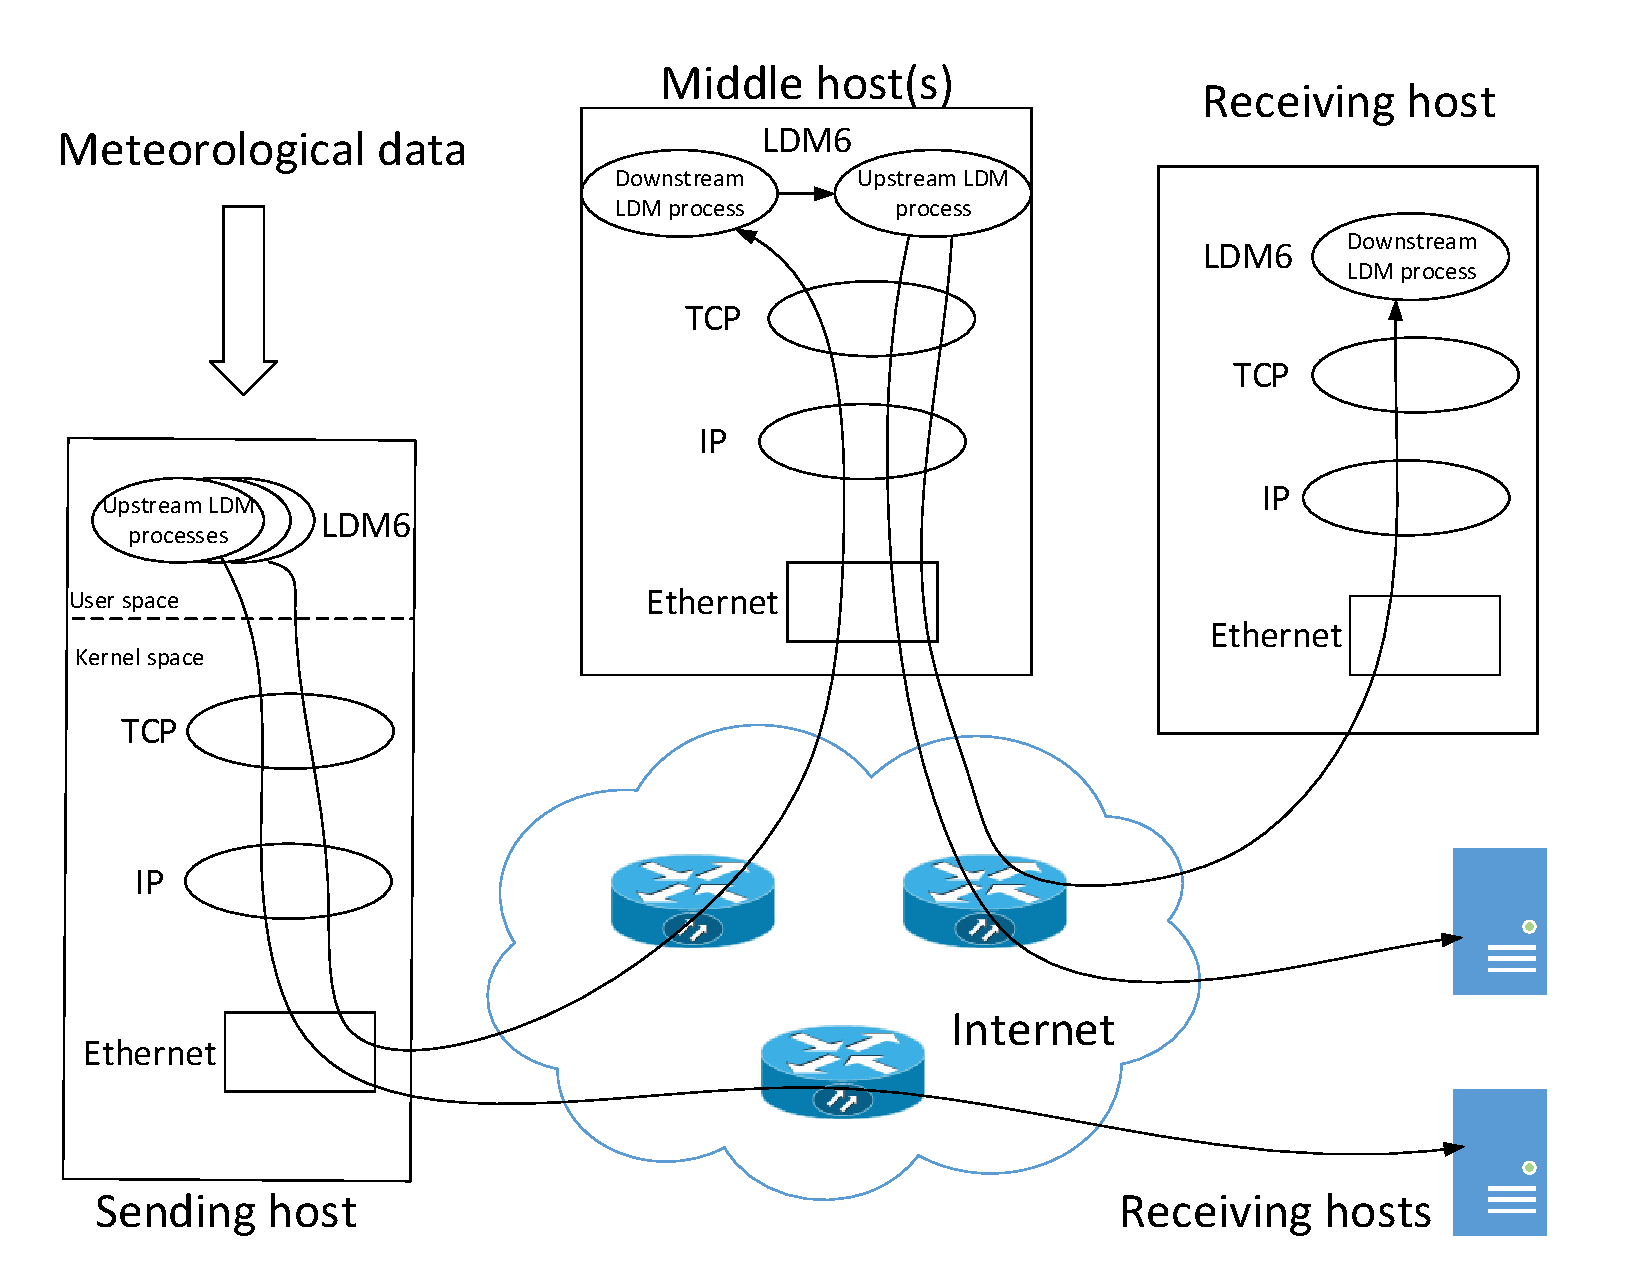
\includegraphics[width=0.60\textwidth]{figures/ALmulticast.pdf}
\caption{LDM6: Application-layer multicasting}
\label{fig:AL-multicast}
\end{figure*} 

\begin{figure*}[htbp!]
\centering
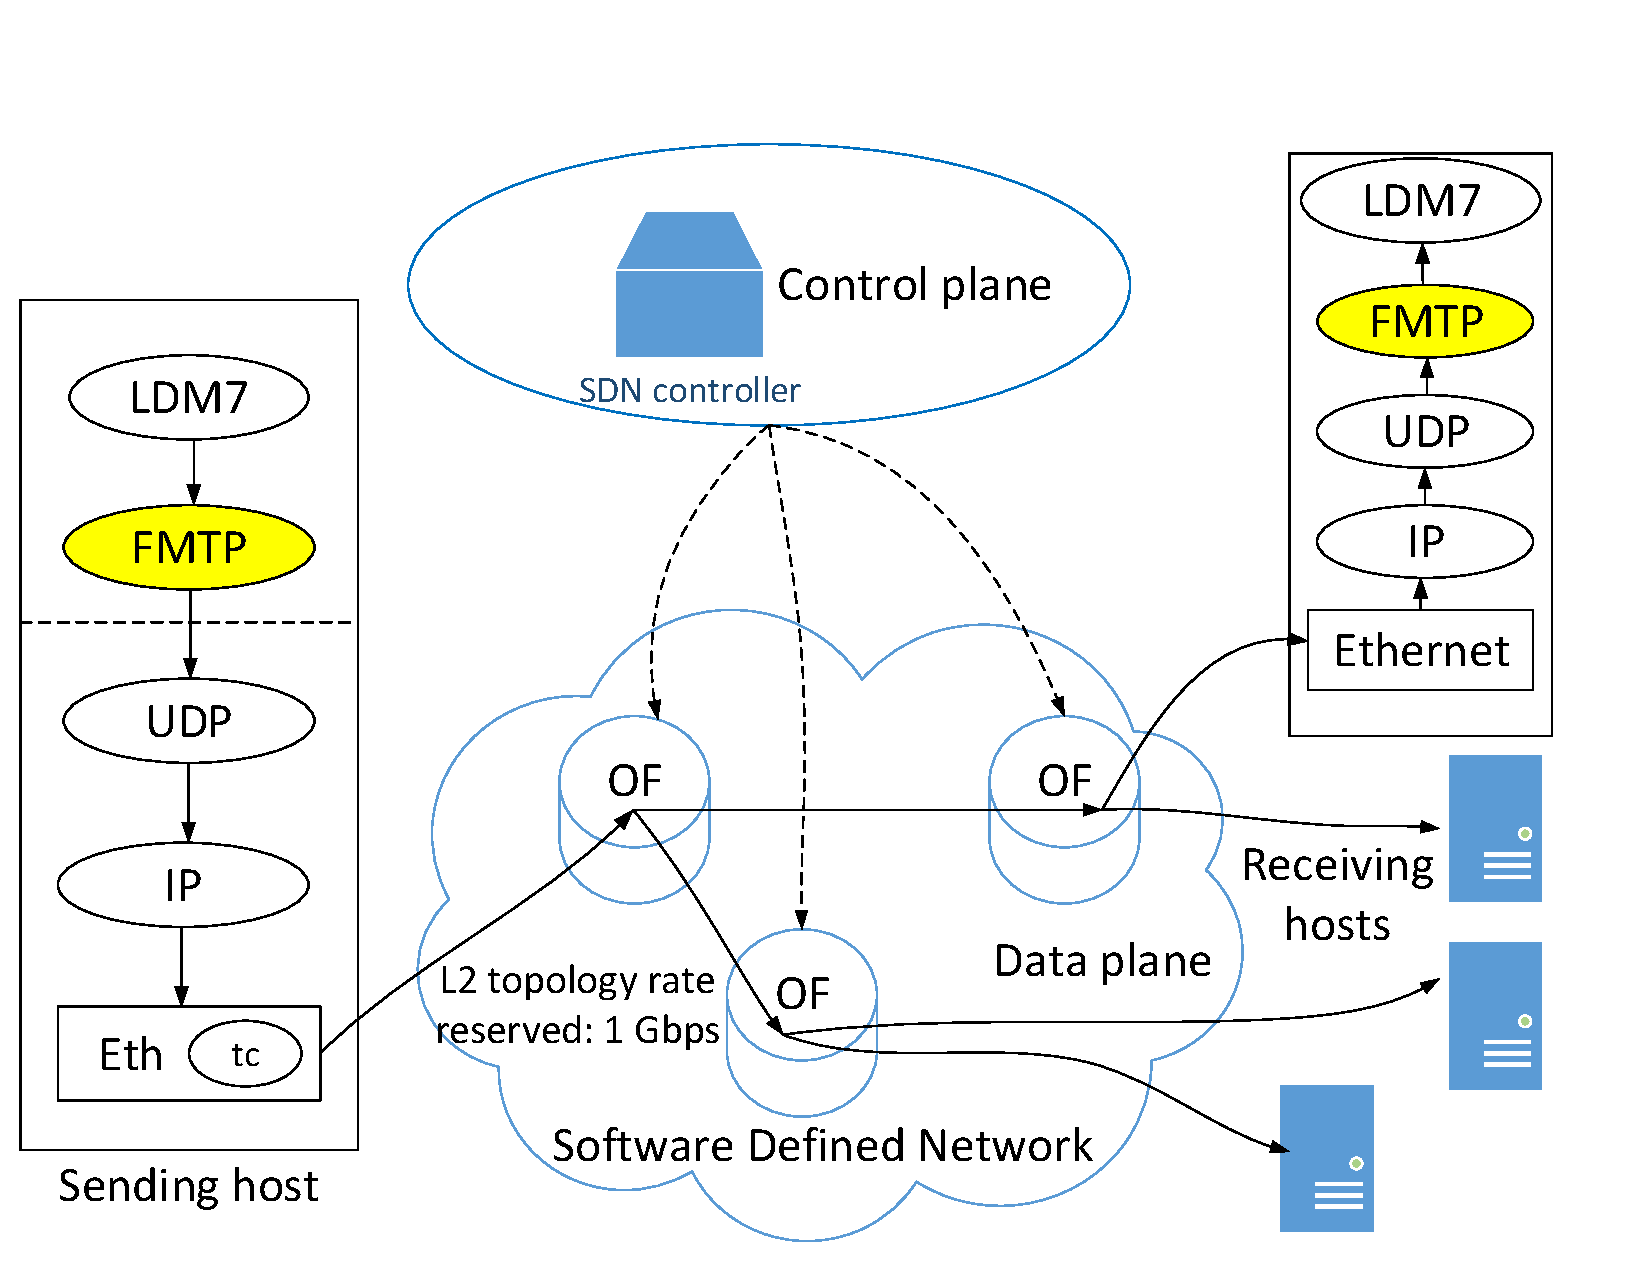
\includegraphics[width=0.60\textwidth]{figures/SDN.pdf}
\caption{LDM7: Layer-2 multicasting across an SDN}
\label{fig:SDN}
\end{figure*} 

\subsection{LDM7 solution for SDN: OpenFlow multicast}
\label{sec:LDM7}
The scalability problem can be solved by a solution in which network switches/routers perform the mulcasting action instead of servers. The availability of OpenFlow/SDN technologies has enabled the deployment of Layer-2 (L2) multipoint virtual topologies.There is a setup phase in which the SDN controller provisions the L2 virtual circuit. This phase is realized by OpenFlow control plane software,Open Exchange Software Suite (OESS) for intra-domain provision, and On-Demand Secure Circuits and Advance Reservation System (OSCARS) for inter-domain provision. Rate guarantees can be provided thus ensuring that there is no differential congestion levels on the paths from the sender to the multiple receivers. Therefore, the LDM7 which integrates the File Multicast Transport Protocol (FMTP) with the current version LDM is implemented for running over OpenFlow/SDN path-based virtual circuits networks, as shown in Fig.~\ref{fig:SDN}.

OpenFlow/SDN networks are now being deployed. For example,
Internet2, a core research-and-education network provider,
has deployed an Advanced Layer-2 Service (AL2S) on top of
a US-wide network of OpenFlow switches \cite{AL2S}.
Through an SDN controller, a multipoint L2 virtual topology can
be configured in the Ethernet switches to multicast Ethernet frames tagged with specific
Virtual LAN (VLAN) identifiers to multiple output ports. Comparing Figs~\ref{fig:AL-multicast} and \ref{fig:SDN}, we see that in the latter,
the OpenFlow switches are making copies of packets to multiple output
interfaces, unlike in the former, where the sending host and
middle hosts make the copies
at the application-layer (LDM6).
OpenFlow 1.3 supports
QoS features, which would allow for the L2 topology to be created with a specific
guaranteed rate. This concept is illustrated in Fig.~\ref{fig:SDN}.
The Linux \texttt{tc} (traffic control) utility can be used to set the rate
at which the Ethernet NIC transmits frames from the sending host. This rate
should be matched to the rate of the L2 multipoint virtual topology created by the
SDN controller. For example, if the NIC is 10 GE, but the rate used
in the setup phase is 1 Gbps, then the \texttt{tc} rate limit should be set to 1 Gbps.

Fig.~\ref{fig:SDN} shows the protocol layers between the application LDM7
and the Ethernet layer. File Multicast Transport Protocol (FMTP) is a reliable multicast transport protocol that we developed for use over rate-guaranteed L2 multipoint virtual topologies \cite{FMTP}.

As noted in Section~\ref{sec:intro}, there are silence periods between files
in the feedtypes. In other words, the file-streams are not continuous. Given
this traffic pattern,
it is challenging to determine an ideal rate for the L2 multipoint virtual topology. If the rate is too low, file-delivery latencies will be high.
If the rate is too high, then other requests for rate-guaranteed paths will be denied by the SDN controller. On the data-plane, QoS mechanisms for packet scheduling
allow the transmitter to send packets from other service classes during silence periods in the LDM file-streams. In other words, network resources are not being wasted during silence periods. This mode of
link sharing is called ``work conserving.'' Nevertheless, there is an incentive to choose a rate that is not too high, to accommodate other users' requests for rate-guaranteed paths. Therefore,
\emph{the problem statement of this thesis is to design a method for computing an ideal rate for the L2 multipoint virtual topology and the size for the buffer at the sending host given the characteristics of the file-stream, and latency and L2 path utilization goals.}
A buffer is used at the sending host to smooth out bursts of file arrivals. 


\section{Characterization of IDD feedtypes}
\label{sec:characterization}


We set up an LDM server on a host at the University
of Virginia (UVA) and configured the server to subscribe to just the
metadata (size and creation-time) for
the top five (from a  rate perspective) feedtypes \cite{IDD_Realtime}.
These are CONDUIT (\texttt{C}), NGRID (\texttt{NG}), NEXRAD2 (\texttt{N2}), NEXRAD3 (\texttt{N3}), and FSL2 (\texttt{F}).
Specifically, the \texttt{notifyme} utility was executed at the UVA LDM server
to receive the metadata for a week (June 2-8, 2014).
The \texttt{notifyme} utility allows a downstream LDM server to receive just the metadata about the files in a feedtype instead of the actual files.
The received metadata
was saved in log files. One entry row is saved in the log file
for each data product of each feedtype. The entry consists of the
creation-time when the product was injected into the IDD system for
distribution (which we refer to as ``arrival time''), and the product size.
The entries in the log files were sorted based on arrival time.
A Python script was implemented
to parse the metadata files and extract the size and arrival
instant of each data product (file).

\begin{table}[!ht]

\caption{Size (in KiB; unless otherwise stated) statistics; June 2, 2014; S: Skewness (R type-1); CV: Coefficient of Variation; M in size: MiB; K and M in last row: $10^3$ and $10^6$, respectively, for number of files.}
\label{tab:size-summary}
\begin{center}
    \begin{tabular}{|l|l|l|l|l|l|}     \hline
    \textbf{Size} & \textbf{\texttt{C}} &  \textbf{\texttt{NG}}  & \textbf{\texttt{N2}} & \textbf{\texttt{N3}} & \textbf{\texttt{F}}\\ \hline
    Min.                             & 0.17          & 0.06  		 & 0.1  		 & 0.15 		 & 0.21\\ \hline
    1st Q		        	      & 10       & 11.8 		& 35.33   		 & 5.18		 & 337.7\\ \hline
    Median                        & 26.7        & 30.3		& 56.3     	 & 9.3		 & 827.4\\ \hline
    Mean                           & 46.24        & 65.29 		& 71.24     	 & 18.88		 & 809.7\\ \hline
    3rd Q		               & 55.3        & 52.1		& 90.9  		 & 22.25		 & 1M\\ \hline
    Max                             & 510.2      & 23.7M    	& 498.5  	 & 206.7		 & 3M\\ \hline
    S		      & 3		 & 28.4	  	& 1.96	   	& 2.42		& 0.85\\ \hline
    CV			      & 1.3		  & 4.9	    	& 0.75	 	& 1.29		 & 0.75\\ \hline
    No.		      & 1.02M   &  526K 	& 1.02M   	& 1.02M	& 36K\\ \hline
\end{tabular}
\end{center}
\end{table}

\begin{table}
    \centering
      \caption{Inter-arrival time statistics; June 2, 2014} \label{tab:inter-arr-time-summary}
\begin{tabular}{|l|l|l|l|l|l|}     \hline
    \textbf{Time (ms)}            & \textbf{\texttt{C}} &  \textbf{\texttt{NG}}  & \textbf{\texttt{N2}} & \textbf{\texttt{N3}} & \textbf{\texttt{F}} \\ \hline
    Min.                             & 0        	   & 0 		& 0	 		 & 0	 		 & 0\\ \hline
    1st Q        	      & 0	           & 4 		& 15	   		 & 2			 & 7\\ \hline
    Median                        & 0	           & 10 		& 36		     	 & 4			 & 16\\ \hline
    Mean                           & 85      	  & 164 		& 85		     	 & 85			 & 2417 ms\\ \hline
    3rd Q                & 1	          & 23 		& 74   		& 11			 & 33\\ \hline
    Max                             & 3687s   & 68s    	& 2382s   	 & 2398s	 & 358s\\ \hline
    S		      & 301.2  & 23.1 	& 333.7   	& 271.3	& 11.6\\ \hline
    CV			      & 91.67  & 13.16    	& 53.10 	& 60.03	& 9.96\\ \hline
    \end{tabular}

\end{table}



\subsection{Size and inter-arrival time data}
\label{sec:size-arrtime}
Five IDD feedtypes are characterized 5 by making the histograms of size and inter-arrival time. We sort the data by ascending order and leave the 25\% data in the end so that the histograms present the distribution better.

% CONDUIT
\begin{figure}
\centering
    \begin{subfigure}{0.5\linewidth}
        \centering
        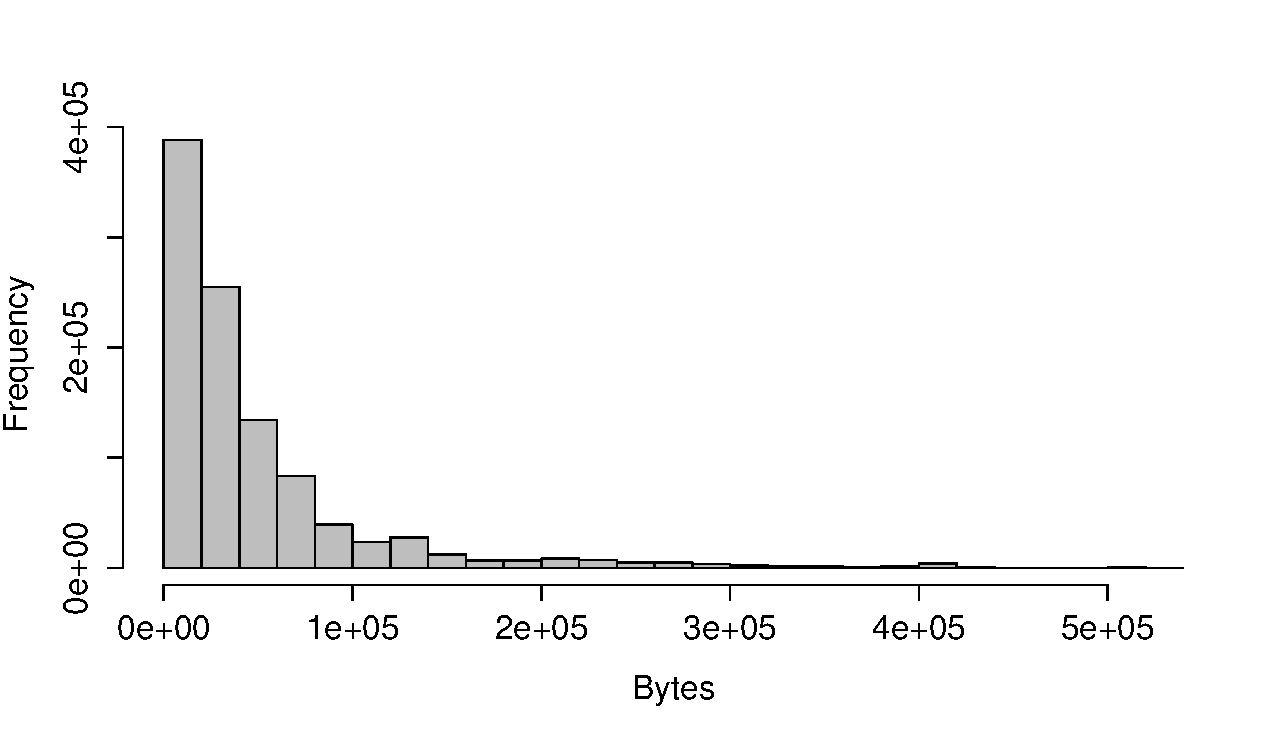
\includegraphics[width=2.2in]{figures/CONDUIT_20140602_Size_Hist.pdf}
        %\includegraphics[width=3.5in]{figures/CONDUIT_Size.eps}
        \caption{Whole size range; Count: 1017621}
        \label{CONDUIT_Size_Whole}
    \end{subfigure}\hfill
    \begin{subfigure}{0.5\linewidth}
	\centering
    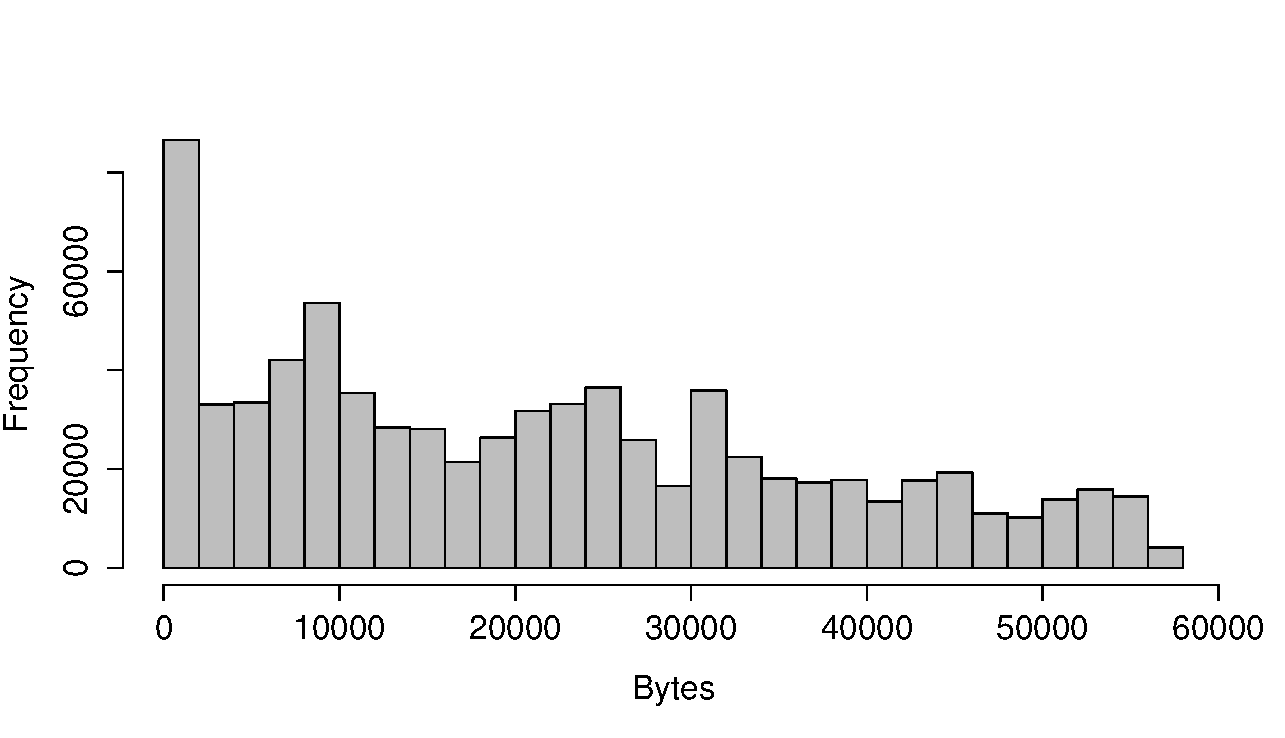
\includegraphics[width=2.2in]{figures/CONDUIT_20140602_Size_75percentile.pdf}
    %\includegraphics[width=3.5in]{figures/CONDUIT-size-75.eps}
        \caption{Top 75 percentile of size range; Count: 763216}
        \label{CONDUIT_Size_75}
    \end{subfigure}\hfill
\caption{Histogram of size of data products sent on June 02, 2014, for the CONDUIT feedtype}
    \label{CONDUIT_Size}
\end{figure}



For all the size and inter-arrival time of feedtypes, the distribution are highly right-skewed.
Fig.~\ref{CONDUIT_Size_75} zooms into the top 75\% data products (from a size perspective). Of the total number of data products, 1017621, as shown
in the last row of Table~\ref{tab:size-summary}, the number of products that fell in the range (0, 20000) bytes (B) was 388,228 (or 38\%). The largest size range (507, 510.2) KiB (1 KibiByte = 1024 B) had 25 data products.
The number of data products in the range (0, 2000) B is 86,520. In other words, 8.5\% of the products were
smaller than 2 KiB, and 38\% of the products were smaller than 20 KiB.

\begin{figure}
\centering
    \begin{subfigure}{0.5\linewidth}
        \centering
        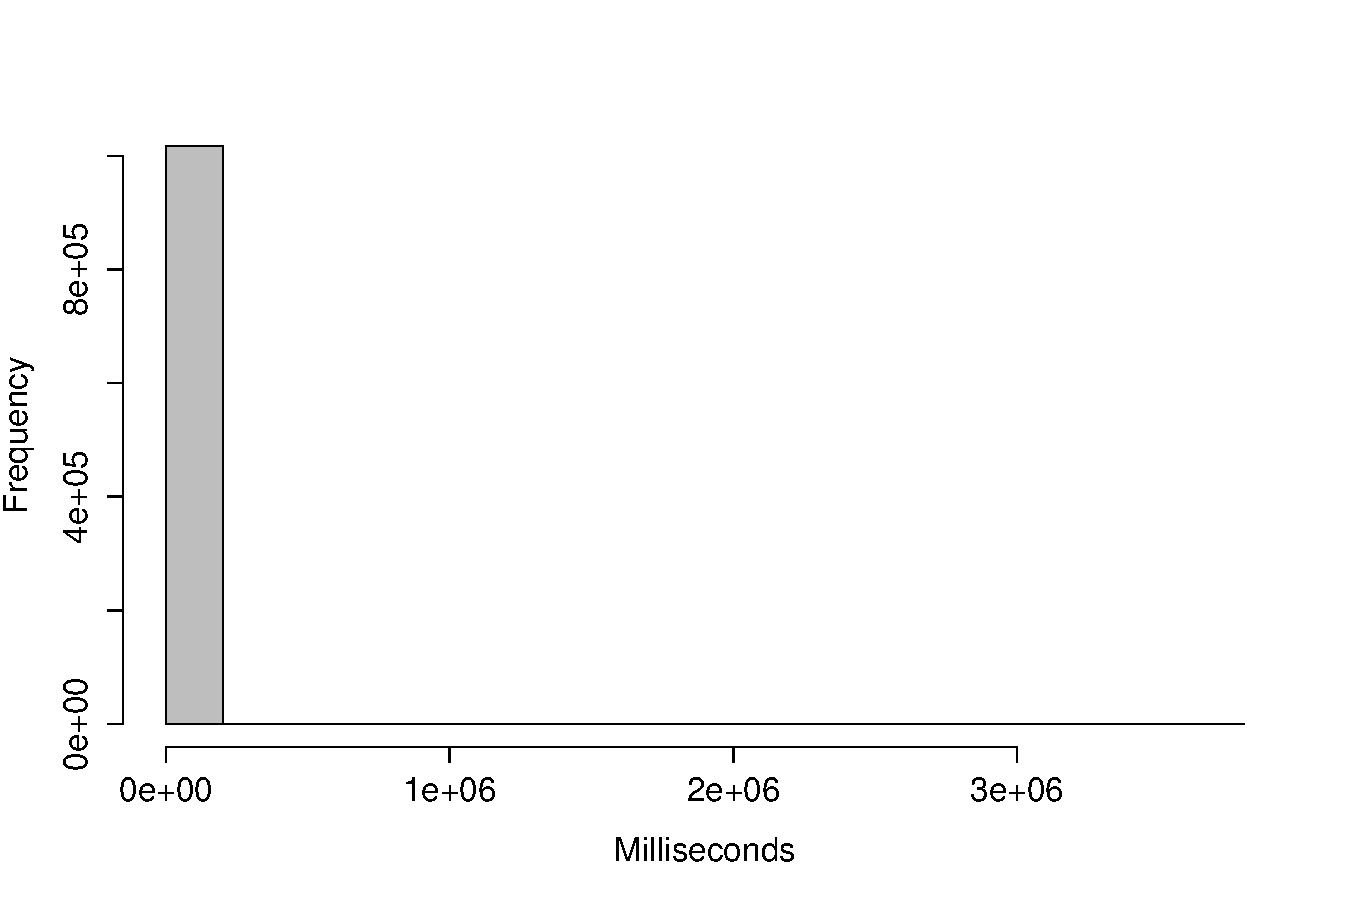
\includegraphics[width=2.2in]{figures/Inter-hist-CONDUIT0602.pdf}
        %\includegraphics[width=3.5in]{figures/CONDUIT_Size.eps}
        \caption{Whole inter-arrival time range; Count: 1017621}
        \label{CONDUIT_Inter_Whole}
    \end{subfigure}\hfill
    \begin{subfigure}{0.5\linewidth}
	\centering
    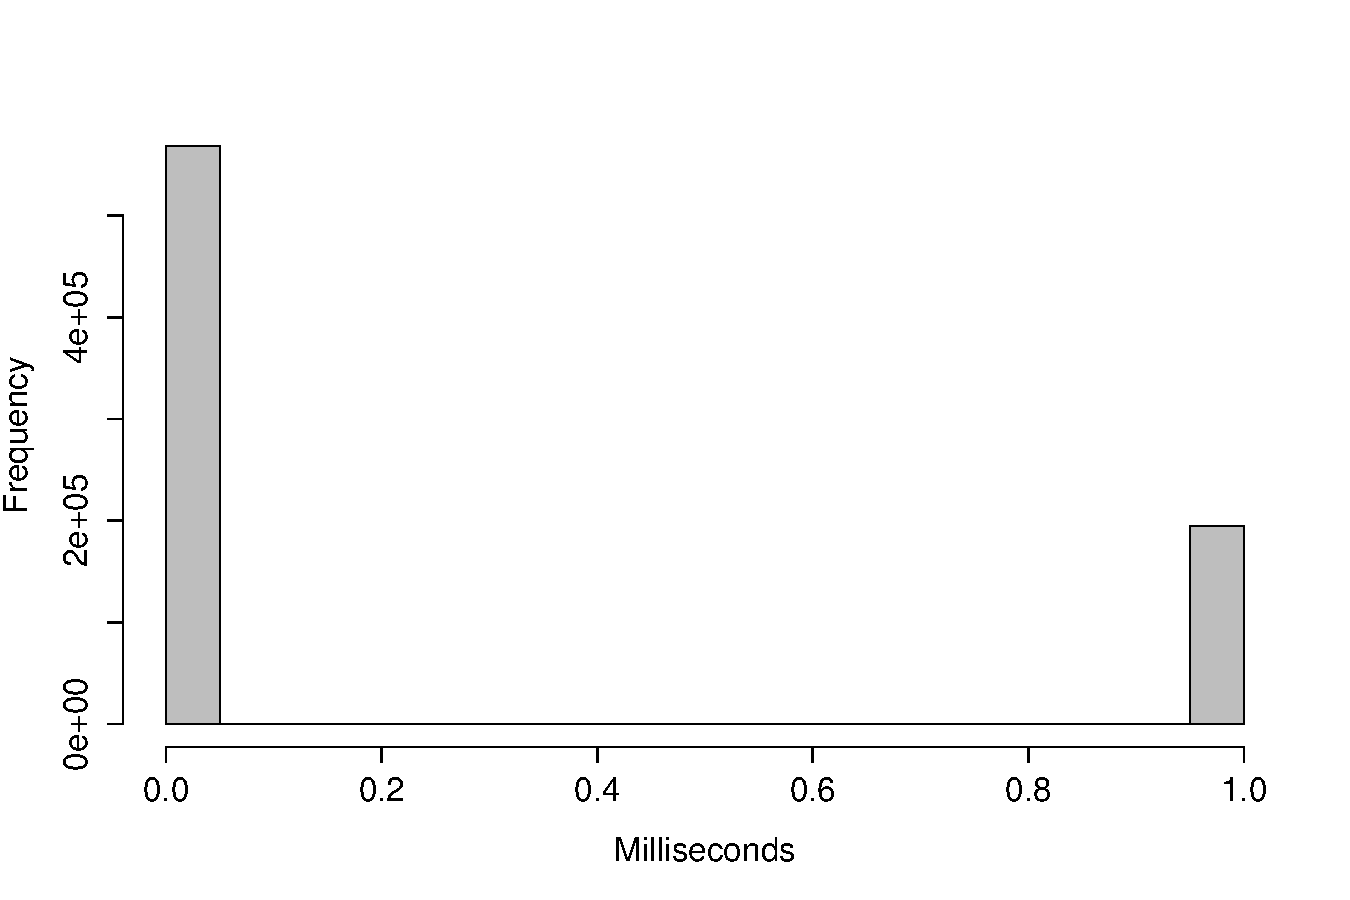
\includegraphics[width=2.2in]{figures/Inter-hist-CONDUIT0602-TOP75.pdf}
    %\includegraphics[width=3.5in]{figures/CONDUIT-size-75.eps}
        \caption{Top 75 percentile of inter-arrival time range; Count: 763216}
        \label{CONDUIT_Inter_75}
    \end{subfigure}\hfill
    \caption{Histogram of inter-arrival time of data products sent on June 02, 2014, for the CONDUIT feedtype}
    \label{CONDUIT_time}
\end{figure}

In the CONDUIT (\texttt{C}) feedtype, over 50\% of the products arrived in the same millisecond as their previous products, i.e., inter-arrival times for
these products was 0 ms (see Table~\ref{tab:inter-arr-time-summary}). Also, the maximum inter-arrival times were
quite large, e.g., maximum silence periods lasted more
than one hour for CONDUIT. (Also see per-min minute average rate figure of CONDUIT feedtype.)
Also, the Top 75\% inter-arrival time histogram indicates that over 25\% inter-arrival time are 1 millisecond.



Tables~\ref{tab:size-summary} and \ref{tab:inter-arr-time-summary} show statistics for sizes and inter-arrival times of data products
distributed in the five feedtypes on June 2, 2014. The NGRID (\texttt{N}) feedtype shows the most skewness for size (see Table~\ref{tab:size-summary}), and the inter-arrival time
coefficient of variation is high for all five feedtypes (see Table~\ref{tab:inter-arr-time-summary}).
Also the maximum-sized data product
is largest for the NGRID feedtype, while FSL2 (\texttt{F}) has the smallest number
of files and the files were generally larger than files in the other feed types.

For significant fractions of an hour
for NEXRAD2 (\texttt{N2}) and NEXRAD3 (\texttt{N3}). For example, as
CONDUIT data is generated by computer models,
this feedtype has silence periods when the models are not being executed.


\subsection{Rate data}
\label{sec:rate-results}
Fig.~\ref{fig:C-rate}, Fig.~\ref{fig:NG-rate}, Fig.~\ref{fig:N2-rate}, Fig.~\ref{fig:N3-rate}, Fig.~\ref{fig:FSL2-rate}  show a plot of per-min average rate, determined
by dividing the aggregate size of all files received in the minute by 60 sec,
as a function of time for 5 feedtypes. Both file-streams
show variable-rate arrivals. There are more silence periods and higher burstiness in the CONDUIT data than in the NGRID feedtype. 
The rate pattern for each day of the same feedtype is similar to each other. This finding is the basis for our problem statement of designing algorithms to determine the sending-host buffer size
and L2 virtual topology rate.

\begin{figure}
\centering
    \begin{subfigure}{0.5\linewidth}
        \centering
        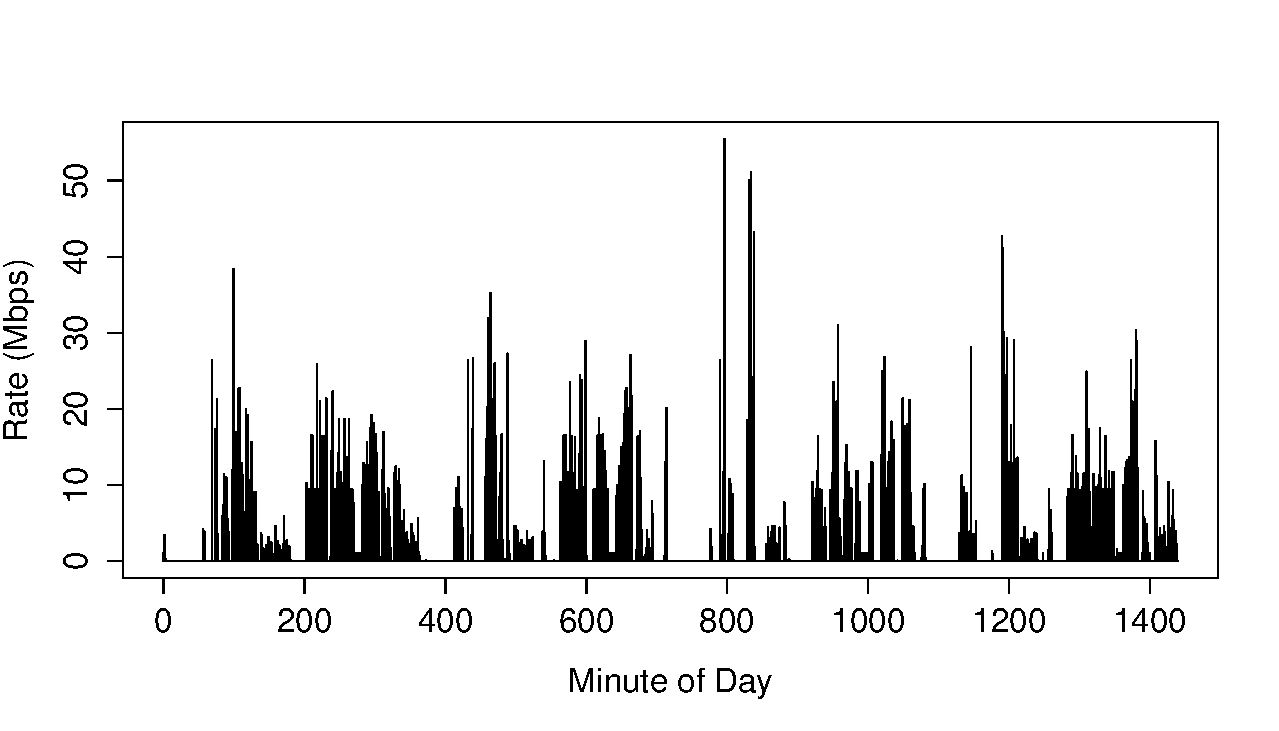
\includegraphics[width=2.2in]{figures/rate_time_CONDUIT0602.pdf}
        %\includegraphics[width=3.5in]{figures/CONDUIT_Size.eps}
        \caption{CONDUIT feedtype}
        \label{fig:C-rate}
    \end{subfigure}\hfill
    \begin{subfigure}{0.5\linewidth}
	\centering
    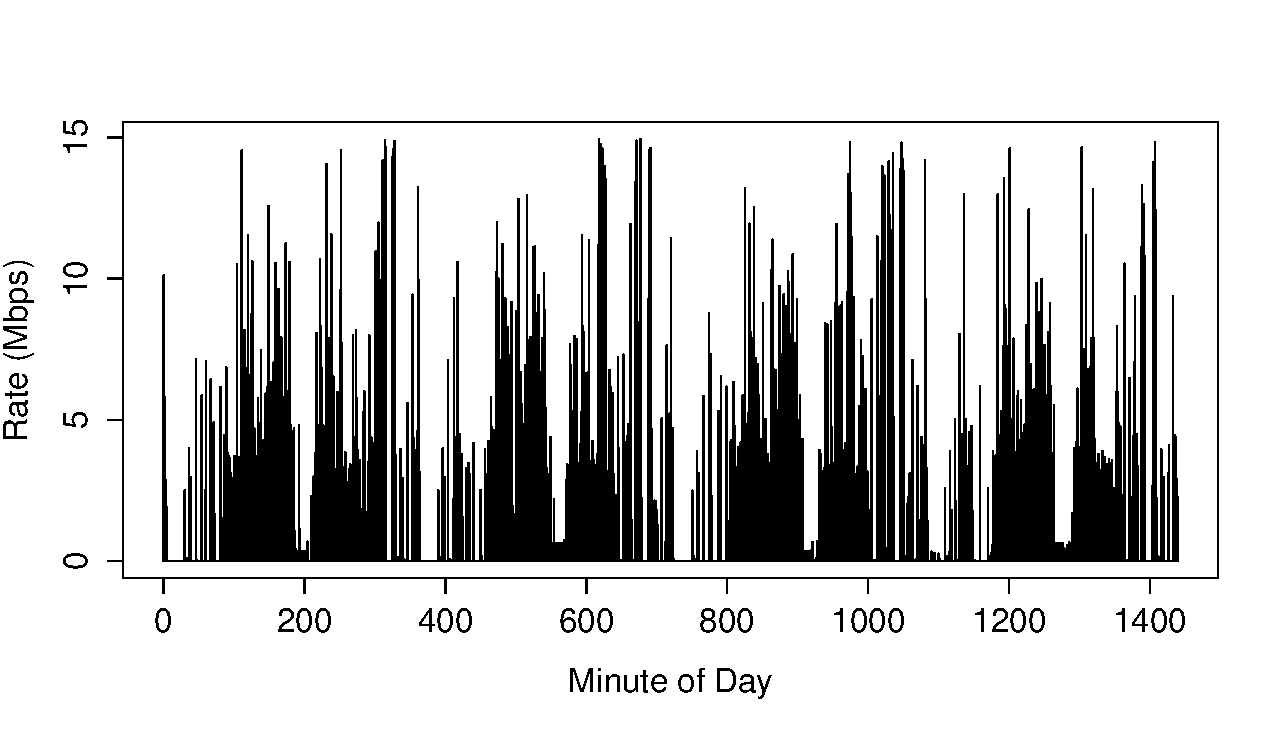
\includegraphics[width=2.2in]{figures/rate_time_NGRID0602.pdf}
    %\includegraphics[width=3.5in]{figures/CONDUIT-size-75.eps}
        \caption{NGRID feedtype}
        \label{CONDUIT_Inter_75}
    \end{subfigure}\hfill
    \caption{Rate vs. time of IDD feedtypes}
    \label{fig:NG-rate}
\end{figure}








\section{Rate selection algorithms for LDM7}
In Section~\ref{sec:LDM7}, we noted that LDM7 is currently
under development, and is designed to use software defined networks.
Further details of
this solution are described in this section.

Fig.~\ref{fig:software} illustrates the LDM7
architecture and operation. The LDM7 server sending host receives
meteorological data at a variable rate. Therefore, we use
a buffer of size $B$ to hold files as the lower protocol layers
(see Fig.~\ref{fig:SDN} for details) divide the files into blocks
and send them to the Ethernet NIC for transmission. The Linux \texttt{tc}
utility is configured to send data at rate $R$, which is equal to the rate
used by the SDN controller to establish the L2 multipoint virtual
topology.

The downstream LDM7 processes are configured to save metadata about the files in a feedtype while receiving the actual files. The metadata is saved in log files. Periodically,
the LDM7 controller shown in Fig.~\ref{fig:software}
reads the log files collected by the receivers, and runs an algorithm,
which is described in Section~\ref{sec:algorithm} to determine the
buffer size $B$ and rate $R$. If the newly computed rate is different
from the rate of the existing L2 multipoint virtual topology, the LDM7 controller
sends a request to the SDN controller to modify the L2 multipoint
virtual topology rate.
Additionally, the LDM7 controller sends a control-plane
message to the LDM7 server in the sending host to reconfigure the Linux \texttt{tc} settings to use the new $R$ value. If the buffer size $B$
also changes, the new buffer size is sent by the LDM7 controller to the sending host as shown in Fig.~\ref{fig:software}.

\begin{figure}
\centering
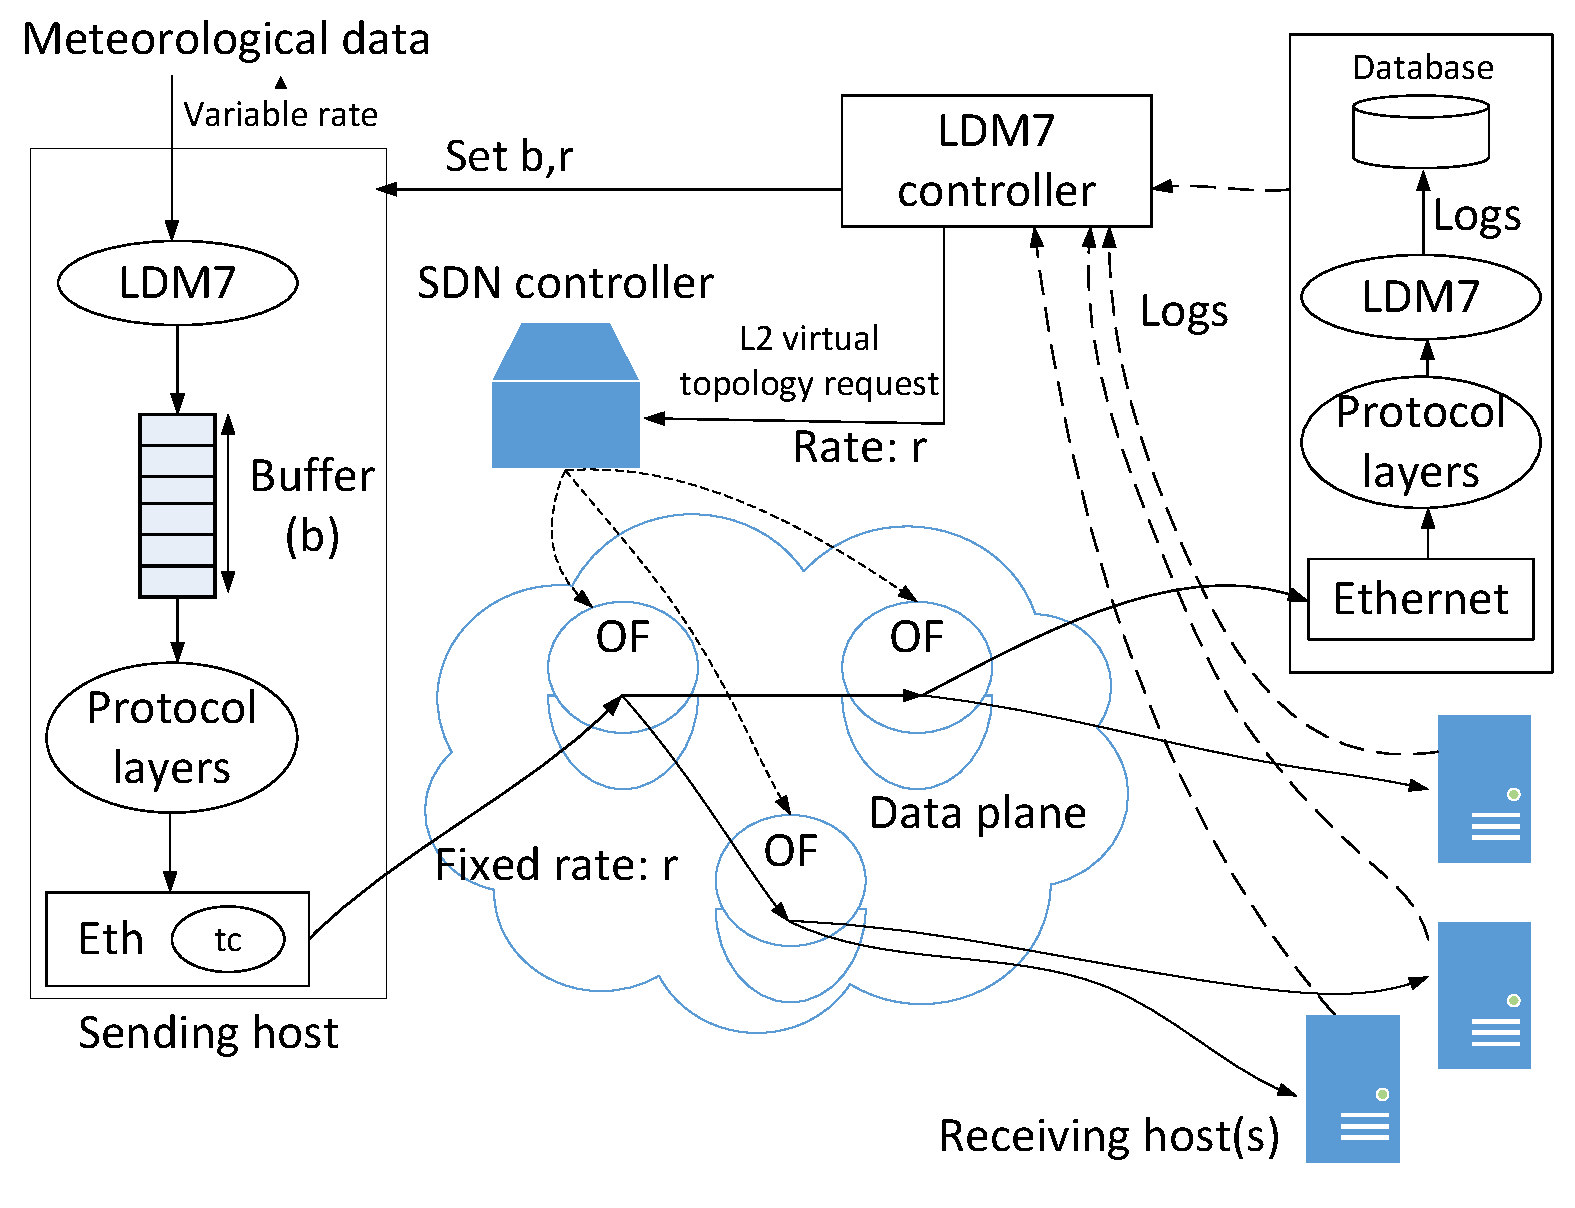
\includegraphics[width=0.5\textwidth]{figures/software.pdf}
\caption{LDM7 architecture and operation}
\label{fig:software}
\end{figure}

\subsection{Algorithms}
\label{sec:algorithm}
The \emph{objective} of the algorithm is to select a rate for the L2 multipoint virtual topology, and a size for the sending-side
buffer, given certain constraints. These constraints are
determined by the method used in the upstream LDM server for
scheduling file transmissions. Since inter-arrival times are short
(see Table~\ref{tab:inter-arr-time-summary}), the upstream LDM
server could be programmed to use of several options for  multiplexing
file transmissions.

In this thesis, we consider two modes: (i) Round Robin (RR), and
(ii) First-Come First Served (FCFS). In RR mode, as new files
arrive, they are immediately added to the buffer, and files in the
buffer are served out one packet at a time.
In FCFS mode, each file is fully transmitted before the next file is served.
In the RR mode, a threshold
$(\mathbb{G},\beta)$ is set such that only
a $\beta$ fraction of files experience multicast throughput less than $\mathbb{G}$.
In the FCFS mode, a wait-time threshold $(\mathbb{W},\alpha)$ is set such that only an $\alpha$ fraction of files experiences a wait time greater than $\mathbb{W}$.

\subsubsection{Overview}

The algorithm
is described for computing and rate and buffer for a single feedtype.
Table~\ref{tab:notation} describes the notation used.
\begin{table*}[!ht]
\centering
\caption{Notation}
\begin{tabular}{|l|p{12.5cm}|}
\hline
\multicolumn{2}{|c|}{Input parameters}\\ \hline
$i$ and $j$ & file indexes\\ \hline
$(t,t+k\tau)$ & $k^{th}$ holding interval \\ \hline
$a_i$ & arrival time of file $i$ \\ \hline
$s_i$ & size of file $i$\\ \hline
\multicolumn{2}{|c|}{System parameters}\\ \hline
$(\mathbb{G},\beta)$ & Fraction $\beta$ of files can experience multicast throughput less than $\mathbb{G}$ in RR mode\\ \hline
$(\mathbb{W},\alpha)$ & Fraction $\alpha$ of files can experience wait times greater than $\mathbb{W}$ in FCFS mode\\ \hline
$r_k$ & configured rate used in the $k^{th}$ holding interval\\ \hline
$b_k$ & configured buffer size used in the $k^{th}$ holding interval \\ \hline
\multicolumn{2}{|c|}{Intermediate values}\\ \hline
$R_k$ & ideal computed rate for the $k^{th}$ holding interval\\ \hline
$B_k$ & ideal computed buffer size for the $k^{th}$ holding interval \\ \hline
$q(t)$ & sending-host buffer (queue) occupancy at time $t$ in ideal case \\ \hline
%$n(t)$ & number of files in the sending-host buffer at time $t$ in ideal case \\ \hline
$d_i$ and $d^{\prime}_i$  & departure time of file $i$, actual and ideal, respectively\\ \hline
$w_i$ and $w^{\prime}_i$ & FCFS wait time experienced by file $i$, actual and ideal, respectively \\ \hline
$g_i$ and $g^{\prime}_i$ & multicast file-transfer throughput of file $i$, actual and ideal, respectively\\ \hline
$\textbf{A}_k$ & set of files that arrived in the $k^{th}$ holding interval \\ \hline
$\textbf{D}_k$ and $\textbf{D}^{\prime}_k $& set of files that departed in the $k^{th}$ holding interval, actual and ideal, respectively \\ \hline
$N_k$ and $N^{\prime}_k $ & number of files that arrived and departed in the $k^{th}$ holding interval, actual and ideal, respectively \\ \hline
$\textbf{M}_k$ and $\textbf{M}^{\prime}_k $ & RR: set of files that experienced multicast throughput lower than $\mathbb{G}$, actual and ideal, respectively\\ \hline
$\textbf{V}_k$ and $\textbf{V}^{\prime}_k $ & FCFS: set of files that experienced wait times greater than  $\mathbb{W}$, actual and ideal, respectively\\
\hline
$\textbf{L}_k$ & set of files that were dropped due to lack of space in the sending-host buffer in the $k^{th}$ holding interval \\ \hline
\multicolumn{2}{|c|}{Output metrics}\\ \hline
$U_k$ & path utilization in the $k^{th}$ holding interval \\ \hline
$\Theta_k$ & mean multicast throughput of files that arrived and departed  in the $k^{th}$ holding interval\\ \hline
$\delta_k$ & dropped file rate in the $k^{th}$ holding interval\\ \hline
$\eta_k$ & RR: throughput-violation rate in the $k^{th}$ holding interval\\ \hline
$\gamma_k$  & FCFS: waiting-time violation rate in the $k^{th}$ holding interval\\ \hline
\end{tabular}
\label{tab:notation}
\end{table*}




First we define a term called \emph{Holding interval}, which is the
period for which the assigned rate and buffer size (as illustrated in
Fig.~\ref{fig:software}) are held unchanged. The $k^{th}$ holding interval is
denoted $(t,t+k\tau)$ in Table~\ref{tab:notation}. The arrival time and
size of file $i$ are denoted $a_i$ and $s_i$, respectively. The file index $i$ is reset to 1 for the first file arriving in each holding interval.

The sizes and arrival times
of all files that arrived and departed in the holding interval are used
to compute the ideal (post-facto) rate $R_k$ and buffer size $B_k$ that should have been used for the $k^{th}$ holding interval, given
the $(\mathbb{G},\beta)$ and $(\mathbb{W},\alpha)$
thresholds, for the RR and FCFS schemes, respectively. The
ideal rate $R_k$ and buffer size $B_k$ values are combined with the current
rate $r_k$ and buffer size $b_k$ that are in use in the $k^{th}$ holding interval to determine rate $r_{k+1}$ and buffer size $b_{k+1}$
for use in the $(k+1)^{th}$ holding interval.
In other words this solution is an empirical method
for determining the rate and buffer size based on traffic characteristics. An Exponential Weighted
Moving Average (EWMA) scheme such as that used for TCP Round-Trip Time (RTT) estimation to compute Retransmission Time Out (RTO) at the TCP sender is used here to modify the rate/buffer setting from one holding
interval to the next.

Table~\ref{tab:notation} lists the thresholds, $(\mathbb{G},\beta)$ and $(\mathbb{W},\alpha)$, and the configured rate $r_k$ and buffer size $b_k$ as system parameters. Next, Table~\ref{tab:notation} lists a number of intermediate values
computed by the algorithm, and the output metrics.
The reader is referred
to Table~\ref{tab:notation} for details of these values
and metrics.

In the next three subsections~\ref{sec:buffer}, \ref{sec:rate-RR}, and \ref{sec:rate-FCFS},
we describe how the ideal buffer size  $B_k$ and ideal rate $R_k$
can be computed post-facto, i.e., with knowledge of sizes and
arrival times of all files received within a holding interval
$(t,t+k\tau)$. Subsection~\ref{sec:output} describes how
the output metrics are computed, and finally Subsection~\ref{sec:EWMA} shows how the rate and buffer
size settings for the next holding interval are set.

\subsubsection{Ideal buffer size computation}
\label{sec:buffer}

Buffer size can be specified using the same notation for both RR and FCFS modes. Using an ideal path rate $R_k$, buffer occupancy at the time of arrival of each
file is as follows:
\begin{eqnarray}
q(a_1) & = & q(t+(k-1)\tau) \nonumber \\
q(a_2) & = & \max\{0, q(a_1)+s_1 - R_k \times (a_2 -a_1)\} \nonumber \\
q(a_i) & = & \max\{0, q(a_{i-1}) +s_{i-1} - R_k \times (a_i -a_{i-1})\}
\end{eqnarray}
The buffer occupancy at the time of arrival of the first file
of the $k^{th}$ holding interval is the buffer occupancy at the starting instant of
the holding interval, which is $(t,t+(k-1) \tau)$.
The buffer would be drained at rate $R_k$ and hence at the time of arrival
of the second file $a_2$, the buffer is either empty, or has some leftover
bytes from the previous files if those files could not be served out completely before the second file of the $k^{th}$ holding interval arrived. Similar reasoning can be
applied to the buffer occupancy at the time of arrival of an arbitrary
file $i$.

To ensure 0 loss in the $k^{th}$ holding interval, the buffer size $B_k$ should ideally be
\begin{equation}\label{eqn:ideal-buffer}
B_k = \max_{1 \leq i \leq \left\vert\textbf{A}_k\right\vert)} q(a_i)
\end{equation}
where $\textbf{A}_k$ is the set of files that arrived in the
$k^{th}$ holding interval as shown in Table~\ref{tab:notation}. The ideal buffer size $B_k$ depends
on the ideal path rate $R_k$, which in turn is selected for the two modes,
RR and FCFS, as described in the next two subsections, respectively.

\subsubsection{Ideal path rate computation in RR mode}
\label{sec:rate-RR}
The algorithm starts with a configured initial value for $R_k$.
If this value is too small, then the minimum multicast throughput
threshold $\mathbb{G}$ will not be met for at least $(1-\beta)$ fraction of the files. Therefore the algorithm keeps increasing $R_k$ until
$(\mathbb{G},\beta)$ is met.
If the starting value chosen for $R_k$ is too large, and this threshold is not exceeded, the algorithm will
keep decreasing $R_k$ until this threshold is violated. In other words, the algorithm finds the minimum $R_k$ value while simultaneously ensuring that not more than a $\beta$ fraction of the files experience a multicast throughput less than $\mathbb{G}$.

The departure times, $d^{\prime}_i$, assuming the ideal
rate and buffer size can be computed by having the algorithm
track packet emission delays. With these departure times,
the ideal multicast file-transfer throughput for file $i$ would be
\begin{equation} \label{eqn:file-throughput}
g^{\prime}_i = \frac{s_i}{(d^{\prime}_i - a_i)}
\end{equation}

Ideal path rate $R_k$ for the $k^{th}$ holding interval is the smallest value at which the following inequality holds:
\begin{equation} \frac{\left\vert{\textbf{M}^{\prime}_k}\right\vert}{N^{\prime}_k}  \le \beta
\end{equation}
where $i \in \textbf{M}^{\prime}_k$ if $g^{\prime}_i < \mathbb{G}$
and $t \leq a_i, d^{\prime}_i \leq t+k\tau$.
The set of files that would have experienced multicast throughput lower than $\mathbb{G}$ in the $k^{th}$ holding interval is $\textbf{M}^{\prime}_k$, and $N^{\prime}_k$ is the number of
files that would have arrived and departed in the $k^{th}$ holding interval, under ideal assumptions of rate and buffer size.
$N^{\prime}_k = \left\vert\textbf{A}_k \cap \textbf{D}^{\prime}_k\right\vert$.


\subsubsection{Ideal path rate computation in FCFS mode}
\label{sec:rate-FCFS}
Each newly arriving file $i$ will experience a waiting
time that is dependent on the buffer occupancy at the time of its arrival $a_i$,
and the ideal path rate $R_k$, since, in
FCFS mode, each file is transmitted in its entirety before
the next file is served.
Thus, waiting time for file $i$ in FCFS mode is:
\begin{equation} \label{eqn:ideal-wait}
w^{\prime}_i = \frac{q(a_i)}{R_k}
\end{equation}
Ideal path rate $R_k$ for the $k^{th}$ holding interval is the smallest value
at which the following inequality holds:
\begin{equation}
\frac{\left\vert\textbf{V}^{\prime}_k\right\vert}{N^{\prime}_k} \leq \alpha
\end{equation}
where $i \in \textbf{V}^{\prime}_k$ if $w^{\prime}_i < \mathbb{W}$
and $t \leq a_i, d^{\prime}_i \leq t+k\tau$.
The set of files that would have experienced wait times in the sending-host buffer greater than $\mathbb{W}$  in the $k^{th}$ holding interval is $\textbf{V}^{\prime}_k$ under ideal assumptions of rate and buffer size.

In FCFS mode, the ideal departure time for file $i$ would be
\begin{equation}\label{eqn:FCFS-wait}
d^{\prime}_i= (w^{\prime}_i + s_i/R_k) + a_i
\end{equation}
where $w^{\prime}_i$ is given by \eqref{eqn:ideal-wait}.

\subsubsection{Output measures}
\label{sec:output}

Five output measures are considered: (i) mean multicast throughput,
(ii) L2 multipoint virtual topology utilization, (iii) dropped-file
rate, (iv) RR: throughput-violation rate and (v) FCFS: waiting-time violation rate. The output measures under the actual rate $r_k$ and
buffer size $b_k$ used in the $k^{th}$ holding interval are computed
below.

The multicast file-transfer throughput for file $i$ is given by
\begin{equation} \label{eqn:file-throughput}
g_i = \frac{s_i}{(d_i - a_i)},
\end{equation}
where $d_i$, the departure time of file $i$, is computed
under RR and FCFS mode assumptions using the actual rate and buffer
size. For example, under FCFS mode, $d_i$ is computed
using \eqref{eqn:FCFS-wait} with
the actual rate $r_k$ instead of the ideal rate $R_k$,
and with $w^{\prime}_i$ replaced by $w_i$, which can be computed
using \eqref{eqn:ideal-wait} but with $r_k$ instead of $R_k$.

The mean multicast throughput for the files that arrived and departed in the $k^{th}$ holding interval is:
\begin{equation}
\Theta_k = \frac{1}{N_k} \sum_{i=1}^{i=N_k} g_i
\end{equation}
where $N_k$ is the actual number of files that arrived and
departed in the $k^{th}$ holding interval, i.e.,
$N_k = \left\vert\textbf{A}_k \cap \textbf{D}_k\right\vert$.
We use the term ``multicast throughput'' instead of the term
``throughput'' as the latter should reflect time for retransmissions,
if any. Packet loss, which can occur at the receiver buffers
even in rate-guaranteed networks, and the corresponding mechanism for retransmssions, are addressed in our reliable multicast transport protocol \cite{FMTP}.

The path utilization in the $k^{th}$ holding interval is given by:
\begin{equation} \label{eqn:util}
U_k \approx \frac{\sum_{i=1}^{i=N_k} s_i}{r_k \times \tau}.
\end{equation}
In other words, utilization is the fraction of time that the path is in use. The reason for the approximate sign is that some parts of the files that were in the sending-side buffer at time $(t+(k-1)\tau)$ (start of the
$k^{th}$ holding interval), and parts of the files that remain in the buffer at time $(t+k\tau)$ (end of the $k^{th}$ holding interval),
would also have been served during
that interval, and therefore the utilization will be greater than
estimated by \eqref{eqn:util}. The longer the holding interval the more
accurate the approximation.

If there is insufficient space in the sending-host buffer to hold file $i$ at the time of its arrival $a_i$, then the file will be dropped, i.e., if
$q(a_i) + s_i > b_k$, the file index $i$ is added to set
$\textbf{L}_k$. Dropped file rate in the $k^{th}$ holding interval is:
\begin{equation}
\delta_k = \frac{\left\vert\textbf{L}_k\right\vert}{N_k}
\end{equation}
With the ideal rate and buffer values
($R_k$ and $B_k$), there will 0 dropped files because the ideal buffer size was selected using \eqref{eqn:ideal-buffer}, but with the actual rate and
buffer settings ($r_k$ and $b_k$), a file will be dropped if
there is insufficient space in the buffer to hold the file
at the time of its arrival.

Similarly with the ideal rate and buffer values, the $(\mathbb{G},\beta)$ and $(\mathbb{W},\alpha)$ thresholds for RR and FCFS, respectively,
will not be violated because these thresholds were considered while determining
the ideal values. However, with the actual rate and buffer size, these thresholds could be violated.
Using sets $\textbf{M}_k$ and $\textbf{V}_k$ to represent the
set of files that experienced multicast throughput lower than $\mathbb{G}$ in the RR mode, and experienced
wait times greater than $\mathbb{W}$ in the FCFS mode, respectively,
we define the RR-mode throughput
violation rate $\eta_k$ and FCFS-mode waiting-time violation rate $\gamma_k$.

RR-mode throughput violation rate is:
\begin{equation}
\eta_k = \frac{\left\vert\textbf{M}_k\right\vert}{N_k}
\end{equation}

FCFS-mode waiting-time violation rate is:
\begin{equation}
\gamma_k = \frac{\left\vert\textbf{V}_k\right\vert}{N_k}
\end{equation}

\subsubsection{EWMA procedure to compute actual rate and buffer size}
\label{sec:EWMA}

An empirical approach is used to compute the L2 multicast path
rate and sending-host buffer size based on the observed metadata
in each holding interval.
Using EWMA, controlled with a weight parameter $W$, the rate used
in the $(k+1)^{th}$ holding interval, $r_{k+1}$ is computed from
the rate  $r_{k}$ used in the $k^{th}$ holding interval, and the ideal
rate, $R_k$, computed for the $k^{th}$ holding interval, as follows:
\begin{equation}\label{eqn:EWMA}
r_{k+1} = \frac{W}{(W+1)} r_k + \frac{1}{(W+1)}  R_k
\end{equation}

%Using EWMA with a weight factor of $\alpha$,
%\begin{equation}
%b_{k+1} = (1-\alpha) b_k + \alpha B_k
%\end{equation}

For the buffer size at the sending host, it is important to
keep dropped-file rate as close to 0 as possible. Therefore,
our approach is to choose the bigger of two values, the buffer
size, $b_k$, used in the $k^{th}$ holding interval, and the newly
computed ideal buffer size, $B_k$, for the buffer size for the next
holding interval. Therefore:
\begin{equation}
b_{k+1} = max(B_k,b_k)
\end{equation}
Administrative procedures can be used to monitor the $b_k$ value
and lower the buffer size if the ideal buffer size computed
on several consecutive holding intervals is considerably lower. 



\section{Numerical results}
The one-week data for the five feedtypes characterized
in Section~\ref{sec:characterization} is used for an application
of the algorithm described in Section~\ref{sec:algorithm}.
Section~\ref{sec:rate-buffer}
shows results
obtained by applying the ideal buffer-size and ideal
rate computation methods, described in Sections~\ref{sec:buffer} and \ref{sec:rate-RR} for the RR-mode,
to one-day's data (holding interval is 1 day) for the five feedtypes. 
Section~\ref{sec:FCFS-RR-comparison} discusses the differences
in results obtained for the ideal buffer size and rate
under the assumptions of RR mode and FCFS mode.
The output metrics, as described in Section~\ref{sec:output},
are presented. Section~\ref{sec:EWMA-results}
presents results for the CONDUIT feedtype
when applying the EWMA method
described in Section~\ref{sec:EWMA} for six consecutive days.

\subsection{Computing ideal rate and buffer size for RR mode}
\label{sec:rate-buffer}

We used threshold values, $\mathbb{G}=10$ kbps, $\beta=0.05$,
to run the RR-mode algorithm first and found the minimum path
rate and buffer size for each of the five
feedtypes using the June 2, 2014 metadata.
Table~\ref{tab:RR-rate-buffer} shows the results.
\begin{table}
\caption{June 2, 2014; Ideal path rate and buffer size in RR mode; $\mathbb{G}=10$ kbps; $\Theta$: mean multicast throughput; $\beta=0.05$}
\centering
\begin{tabular}{| c | p{0.5in} | p{0.4in} | p{0.3in} |p{0.6in}|} \hline
Feedtype & Rate (Mbps) & Buffer size (MiB) & Util. (\%) & $\Theta$ (kbps)\\ \hline
CONDUIT & 36 & 248 & 12.4 & 535.2 \\ \hline
NGRID &10 & 315 & 32.6 &436.6  \\ \hline
NEXRAD2 & 16& 38 &42.9 &7370.2   \\ \hline
NEXRAD3 &6 & 19 &30.4 &661.6 \\ \hline
FSL2 & 4 & 306 &68.6 &54.4  \\ \hline
% FSL2 (G=20) & 6 &244 &45.7&119.3  \\ \hline
\end{tabular}
\label{tab:RR-rate-buffer}
\end{table}
The ideal rate computed for the CONDUIT feedtype is 36 Mbps,
and the ideal buffer size is 248 MiB. Had these rate and buffer
settings been used, no files would have been dropped.

The utilization and mean multicast throughput values shown
in Table~\ref{tab:RR-rate-buffer} are computed using the methods
described in Section~\ref{sec:output} but with the ideal rate and buffer
size settings, not the actual rate and buffer size settings as described
in that section. In other words, the mean multicast throughput across the 1.02 M files (see last row
of Table~\ref{tab:size-summary}) received that day for the CONDUIT feedtype
would have been 535.2 kbps had the ideal rate and buffer settings been used. The L2 multicast path would have been
only utilized at only 12.4\%.
As noted in Section~\ref{sec:LDM7}, utilization is not a concern per-se
because the link is shared in work-conserving mode. The CONDUIT traffic
is bursty (see Fig.~\ref{fig:C-rate}), and therefore, 36 Mbps is the smallest rate at which the
$(\mathbb{G},\beta)$ threshold values can be met. On the other hand,
the utilization of a 4 Mbps path is 68.6\% for the FSL2 feedtype
as seen in the last row of Table~\ref{tab:RR-rate-buffer}.

\subsection{Comparing the two modes, RR and FCFS}
\label{sec:FCFS-RR-comparison}
We executed the FCFS-mode algorithm described in Sections~\ref{sec:buffer} and ~\ref{sec:rate-FCFS} to find the ideal buffer size and rate. For
the FCFS $(\mathbb{W},\alpha)$ constraint, we assumed
$\alpha=0.2$, but experimented with different values of
$\mathbb{W}$ until we found a setting
for which the mean multicast throughput $\Theta$ values were approximately the same as those computed by the RR-mode
algorithm and shown in Table~\ref{tab:RR-rate-buffer}.

Table~\ref{tab:FCSF-rate-buffer} shows the computed
values of $\mathbb{W}$, ideal rate and ideal buffer size, using June 2, 2014 metadata.
\begin{table}
\caption{June 2, 2014; Ideal path rate and buffer size in FCFS mode; $\Theta$: mean multicast throughput; $\alpha = 0.2$}
\centering
\begin{tabular}{| c| p{0.25in} | p{0.4in} | p{0.4in} | p{0.3in}| p{0.5in}|} \hline
Feedtype & $\mathbb{W}$ (s) & Rate (Mbps) & Buffer size (MiB) & Util. (\%) & $\Theta$ (kbps)\\ \hline
CONDUIT  & 15 &26 &348 & 17 & 543 \\ \hline
NGRID &34 &10 &330 & 33 &604  \\ \hline
NEXRAD2 &1 & 16&49 &43 &8490   \\ \hline
NEXRAD3 &16&6 & 17 &30 &744  \\ \hline
FSL2 &145&6 & 255 &46 &258  \\ \hline
\end{tabular}
\label{tab:FCSF-rate-buffer}
\end{table}
Since this is the ideal rate/buffer size computation, no files are dropped
and the threshold values are met. The
output metrics, utilization and mean multicast throughput ($\Theta$), are
also shown in Table~\ref{tab:FCSF-rate-buffer}.

A comparison of Tables~\ref{tab:RR-rate-buffer} and \ref{tab:FCSF-rate-buffer} shows that for the \emph{NGRID}, \emph{NEXRAD2} and \emph{NEXRAD3} feedtypes, the rate and buffer size values computed for RR mode and FCFS mode are approximately the same. Utilization and mean multicast throughput values are also similar.

For the \emph{CONDUIT} feedtype, the RR mode requires a higher path rate to achieve approximately
the same mean multicast throughput as the FCFS mode. Studying the inter-arrival time
distribution for CONDUIT from Table~\ref{tab:inter-arr-time-summary}, we see
that more than 50\% of the files arrived at the same millisecond as their previous files. Since all files in the buffer are served simultaneously in RR mode, to ensure
that the percent of files for which the multicast throughput is less than $\mathbb{G}$ does not exceed $\beta$, a higher path rate is required.

Finally, for the \emph{FSL2} feedtype, the ideal rate (4 Mbps) and buffer size (306 MiB) computed for the RR mode resulted in a much lower mean multicast throughput (54.4 kbps) than the mean
throughput (258 kbps) obtained at the ideal rate (6 Mbps) and buffer
size (255 MiB) values computed for the FCFS mode.
There is less skew in
the size distribution for FSL2 than in the other feedtypes, files are
generally larger, and spread in inter-arrival times is small (coefficient
of variation at 9.96, as seen in Table~\ref{tab:inter-arr-time-summary}, is the smallest among all feedtypes). These characteristics
make FCFS a better choice for FSL2.

\begin{figure}
\centering               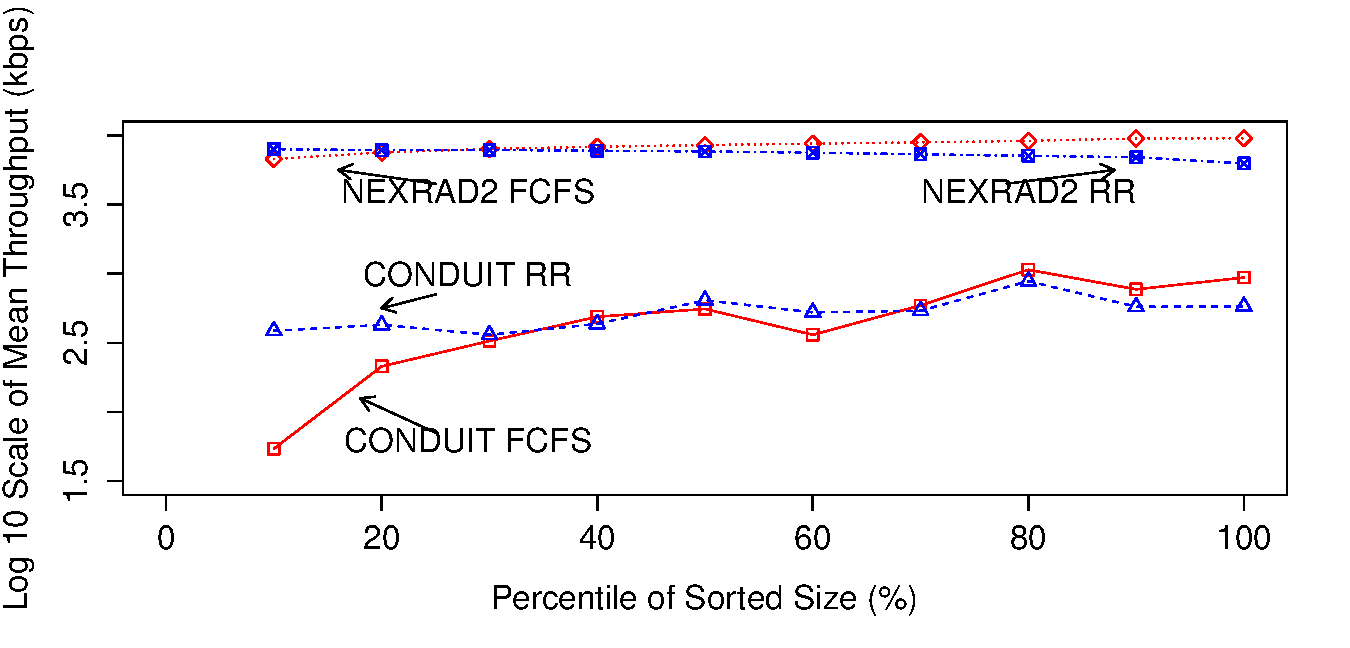
\includegraphics[width=0.5\textwidth]{figures/FCFS-vs-RR.pdf}
\caption{A comparison of per-bin mean multicast throughput values where each bin has 10\% of the files sorted by size}
\label{fig:FCFS-vs-RR}
\end{figure}

The utilization levels in Tables ~\ref{tab:RR-rate-buffer} and \ref{tab:FCSF-rate-buffer} are low, but as explained in Section~\ref{sec:LDM7}, packet scheduling
can be configured to operate in work-conserving mode, which means
that if the queue serving packets for a provisioned path is empty, the scheduler
will serve best-effort IP packets. The L2 path service is offered
on the same infrastructure as best-effort IP service in university campuses
and RENs. Therefore, network resources are not wasted during silence periods in the file-streams.

Finally, to gain a further understanding of FCFS and RR modes, we studied mean multicast throughput as a function of file size by dividing the size range
into 10 bins such that all bins had an equal number
of files. The per-bin mean multicast throughput values
for two feedtypes, CONDUIT and NEXRAD2, are plotted against size
percentile in Fig.~\ref{fig:FCFS-vs-RR}. As expected, smaller files fare better
in the RR mode, while larger files fare better in the FCFS mode
as can be seen in Fig.~\ref{fig:FCFS-vs-RR}. 

\subsection{Application of EWMA method for multiple days}
\label{sec:EWMA-results}
The EWMA scheme described in Section~\ref{sec:EWMA} is applied
to the week-long data for the CONDUIT feedtype when served using the RR mode. But before presenting the results computed using the actual rate
and buffer size set with the EWMA scheme,
Table~\ref{tbl:ideal-week} shows the ideal rate and buffer
size that should have been used each day. These numbers
are computed using the methods described in Sections~\ref{sec:buffer} and \ref{sec:rate-RR}.
\begin{table}[ht]
\caption{Ideal RR rate and buffer size computed with each day's data (post-facto); $\mathbb{G}=10$ kbps; $\beta=5\%$}
\centering
\begin{tabular}{| c | p{0.4in} | p{0.3in} | c | c| c |} \hline
Date & Rate (Mbps) & Buffer size (MiB) & Util. (\%) &  $\Theta$ (kbps) & $\eta_k$ (\%)\\ \hline
June 2 & 36 &248 & 12.4 & 535.2 &4.8 \\ \hline
June 3 & 30 & 362 & 14.3 &270.0 &4.8 \\ \hline
June 4 & 30&269 &15.0 & 424.7 & 4.9 \\ \hline
June 5 &30 & 249 &15.8 &695.5 &4.6 \\ \hline
June 6 &24 & 244 &18.6 &360.3 &4.6 \\ \hline
June 7 & 30 & 290 & 15.0 &514.1 & 4.8 \\ \hline
June 8 & 26 & 244& 16.8 &382.4 & 4.9 \\ \hline
\end{tabular}

\label{tbl:ideal-week}
\end{table}
In all rows of Table~\ref{tbl:ideal-week}, the RR throughput-violation rate
$\eta_k$ is smaller than the threshold $\beta$ value of 5\%.
The ideal rates computed for each day varies as the CONDUIT
model data is not exactly the same from day-to-day. Also, we see
a variation in the ideal buffer size required at the sending host
to achieve 0 loss. The utilization and mean multicast throughput values shown
in Table~\ref{tbl:ideal-week} are computed using the methods
described in Section~\ref{sec:output} but with the ideal rate and buffer
size settings, not the actual rate and buffer size settings.

Next, we present results from the application of the EWMA scheme
of Section~\ref{sec:EWMA}.
Two values of $W$ in \eqref{eqn:EWMA} are used to generate numerical
results.
Table~\ref{tbl:yesterday} shows results when $W=0$ and Table~\ref{tbl:W7} shows results
when $W=7$. With $W=0$, the ideal rate computed in the $k^{th}$ holding
interval is used directly in the $(k+1)^{th}$ holding interval.
With $W=7$, the ideal rate computed is given a weight of 0.125, while the running average rate is given a weight of 0.875.
\begin{table}
\caption{System performance with rate and buffer size computed using EWMA with $W=0$}
\centering
\begin{tabular}{| c | p{0.4in} | p{0.3in} | p{0.3in} | p{0.3in}| p{0.3in} |p{0.3in}|} \hline
Date & Rate (Mbps) & Buffer size (MiB) & Util. (\%) &  $\Theta$ (kbps) & $\eta_k$ (\%) & $\delta_k$ (\%)\\ \hline
June 3 & 36 & 248 & 12.0 &397.2 &3.2 &0.034\\ \hline
June 4 & 30 &362 &15.0 & 424.7 & 4.9&0 \\ \hline
June 5 &30 &362 &15.8 &695.5 &4.6&0 \\ \hline
June 6 &30 & 362 &14.9 &591 &3.4&0 \\ \hline
June 7 & 24 & 362 & 18.8 &309 & 7.2 &0.037\\ \hline
June 8 & 30 & 362& 14.6 &536 & 3.9 &0\\ \hline
\end{tabular}
\label{tbl:yesterday}
\end{table}
\vspace{-0.1in}
\begin{table}[!ht]
\centering
\caption{System performance with rate and buffer size computed using EWMA with $W=7$}
\begin{tabular}{| c | p{0.4in} | p{0.3in} | p{0.3in} | p{0.3in}| p{0.3in} |p{0.3in}|} \hline
Date & Rate (Mbps) & Buffer size (MiB) & Util. (\%) &  $\Theta$ (kbps) & $\eta_k$ (\%) & $\delta_k$ (\%)\\ \hline
June 3 & 36 & 248 & 12.0 &397.2 &3.2 &0.034 \\ \hline
June 4 & 35.3&362 &12.7 & 598.7 & 4.3&0 \\ \hline
June 5 &34.6 & 362 &13.7 &952.2 &3.7 &0\\ \hline
June 6 &34 & 362 &13.1 &780 &2.6&0 \\ \hline
June 7 & 32.8 & 362 & 13.8 &626 & 4.1&0 \\ \hline
June 8 & 32.4 & 362& 13.5 &643 & 3.8&0 \\ \hline
\end{tabular}

\label{tbl:W7}
\end{table}

In Table~\ref{tbl:yesterday}, we see that the rate used for June 3, which is 36 Mbps, is the  ideal rate computed for June 2, as seen in Table~\ref{tbl:ideal-week}. A similar pattern is observed in subsequent rows when comparing rates of Tables~\ref{tbl:ideal-week} and \ref{tbl:yesterday}. The
buffer size in Table~\ref{tbl:yesterday} increases to 362 MiB, but
stays at that level, which means the traffic on subsequent days did
not cause a larger backlog than it did on June 4. The only day
in which the EWMA scheme with $W=0$ violated the RR throughput-violation
rate is on June 7, when $\eta_k$ reached 7.2\%, exceeding the $\beta$
threshold of 5\%. Correspondingly, there were dropped files, with the dropped-file rate $\delta_k$ reaching 0.037\%. For
all days, the actual rates used, as indicated in Table~\ref{tbl:yesterday}
are higher or equal to the ideal rates presented in
Table~\ref{tbl:ideal-week}, except for June 7, when the ideal rate
was 30 Mbps, but the actual rate used was only 24 Mbps.

The second $W$ setting of 7 worked well. On June 7, as seen in Table~\ref{tbl:W7}, the actual rate used was 32.8 Mbps, while
the ideal rate as seen in Table~\ref{tbl:ideal-week} was only 30 Mbps.
Table~\ref{tbl:W7} shows that there were dropped files ($\delta_k = 0.034\%$) on June 3, which being the first day, did not have the benefits of rate averaging and buffer maximization.


The results presented here are examples of how the EWMA scheme works.
In a practical deployment, the particular $W$ value will need to be
selected for each feedtype, as the day-to-day variation in traffic
depends on the feedtype.

\section{Related work}
A MultiPath MultiCast (MPMC) algorithm to distribute a file to multiple receivers, with segments of files being transmitted
on multiple paths, is proposed and evaluated on OpenFlow networks \cite{6630542}.
The problem statement of this work is different from ours, i.e., unlike in our work, path rate computation is not an objective in the MPMC algorithm development.

A paper on Layer-2 multicast in OpenFlow networks for multimedia distribution
(VLC streaming) \cite{6799481} compares the ease of using of OpenFlow-enabled
Layer-2 multicasting with IP multicasting and application-layer multicasting.
The path setup phase in OpenFlow-controlled L2 multicasting negates the need for distributed multicast routing protocols, which has proven to be challenging but necessary for IP multicasting. A method for dynamic path adjustment of OpenFlow-controlled multicast trees is presented by Ge et al. \cite{6681003}.

An interesting use of OpenFlow control to isolate elephant flows, which are termed ``significant flows'' and hence worthy of per-flow setup actions, was proposed \cite{Curtis:2011:DSF:2018436.2018466}. It is related to our work because it uses OpenFlow for path setup for particular flows, but the issue of rate computation is not addressed.
The use of QoS controls in OpenFlow networks is explored in a testbed \cite{6385057}, and proposed for video streaming \cite{6116083}.

Finally seminal work on how to compute rate for a virtual circuit
for a given traffic model was done by Guerin et al. \cite{103545}.
This work was applied for audio and video streams for which the modeling
assumptions held. These assumptions do not hold for our file-stream traffic. 

\section{Summary and conclusions}
This work identified an exciting new problem
of rate determination for L2 multipoint virtual topologies
to serve variable-rate file streams to multiple receivers. Prior work
on rate computation methods were designed for audio/video
streams, not file streams. The problem is based on the need
for scalability in a real deployment as data volumes and
number of receivers have grown. Our solution was based, not
on models, but on actual traffic characteristics. These
characteristics, such as right-skewed file size and file
inter-arrival times, and variability from day-to-day,
are likely to hold for other types of file-streams. 
Our solution, based on a empirical method and an exponential weighted moving average scheme, was designed
to have broad applicability, not customized for the IDD feedypes.
Evaluation of our method with real traffic (from five IDD feedtypes) showed that
while throughput constraints can be met by selecting a suitably high
rate, utilization varies based on the burstiness of each file-stream.
However, if rate-guaranteed L2 services are offered
on the same network as best-effort IP services, and packet schedulers
are configured to operate in work-conserving mode, the utilization levels
of the L2 multipoint topologies are not of significant concern.
